%\documentclass{ucbthesis}
%\usepackage{amssymb}
%
%\usepackage{color}
%\usepackage{amsmath}
%\usepackage{enumerate}
%\usepackage{caption}
%\usepackage{subcaption}
%\usepackage{amsthm}
%\usepackage{exscale}
%\usepackage[mathscr]{eucal}
%%\usepackage{bm}
%%\usepackage{eqlist} % Makes for a nice list of symbols.
%\usepackage[]{graphicx}
%%\DeclareGraphicsExtensions{.pdf, .jpg, .png}
%\usepackage{natbib}
%%\usepackage{har2nat}
%\usepackage{verbatim}
%\usepackage{url}
%%\usepackage{longtable}
%\usepackage{mathpazo}

%\usepackage{pstricks}
%\usepackage{sgamevar}
%\usepackage{egameps}
%\usepackage{listings}
%
%\usepackage{booktabs} %for top, middle and bottomline
%\usepackage{array} %enables, for table columns, m{width} and b{width} (only p{width is available without it})
%\usepackage{tabularx} %for automation of column widths so that the table spans the width defined by textwidth and linewidth

\documentclass{ucbthesis}
\usepackage[]{graphicx}
\usepackage{epstopdf}
\usepackage{mathrsfs}
\usepackage{amssymb}
\usepackage{color}
\usepackage{amsmath}
\usepackage{enumerate}
\usepackage{braket}
\usepackage{tabularx} %for automation of column widths so that the table spans the width defined by textwidth and linewidth
\usepackage{subcaption}
\usepackage{cite}
\usepackage{appendix}

%\usepackage{notoccite}
\setlength{\overfullrule}{0pt}
\newcommand{\irow}[1]{
  \begin{smallmatrix}(#1)\end{smallmatrix}%
} %inline row vectors

% make the bibliography a section rather than a chapter
%\makeatletter
%\renewenvironment{thebibliography}[1]
%     {\section*{\bibname}
%      \@mkboth{\MakeUppercase\bibname}{\MakeUppercase\bibname}%
%      \list{\@biblabel{\@arabic\c@enumiv}}%
%           {\settowidth\labelwidth{\@biblabel{#1}}%
%            \leftmargin\labelwidth
%            \advance\leftmargin\labelsep
%            \@openbib@code
%            \usecounter{enumiv}%
%            \let\p@enumiv\@empty
%            \renewcommand\theenumiv{\@arabic\c@enumiv}}%
%      \sloppy
%      \clubpenalty4000
%      \@clubpenalty \clubpenalty
%      \widowpenalty4000%
%      \sfcode`\.\@m}
%     {\def\@noitemerr
%       {\@latex@warning{Empty `thebibliography' environment}}%
%      \endlist}
%\makeatother

% double spacing: uncomment following lines
\def\dsp{\def\baselinestretch{2.0}\large\normalsize}
\dsp

% paragraph indents: uncomment following line
% \usepackage{indentfirst}

\begin{document}

% Declarations for Front Matter

\title{Thesis Title}
\author{Author}
\degreesemester{Graduation Semester}
\degreeyear{Graduation Year}
\degree{Doctor of Philosophy}
\chair{Major adviser}
\othermembers{Prof. Committee 1 \\ Prof. Committee 2}
\numberofmembers{2}
\field{Physics}
\campus{Amherst}

% For a masters thesis, replace the above \documentclass line with
% \documentclass[masters]{ucbthesis}
% This affects the title and approval pages, which by default calls this
% document a "dissertation", not a "thesis".

\maketitle
% Delete (or comment out) the \approvalpage line for the final version.
% \approvalpage
% \copyrightpage



\begin{frontmatter}

% \begin{dedication}
% \null\vfil
% \begin{center}
% To person\\\vspace{12pt}
% the dedication goes here
% \end{center}
% \vfil\null
% \end{dedication}

% Place acknowledgments below.
\section*{Acknowledgements}
Hello darkness, my old friend
I've come to talk with you again
Because a vision softly creeping
Left its seeds while I was sleeping
And the vision that was planted in my brain
Still remains
Within the sound of silence


\tableofcontents
% \clearpage
% \listoffigures
% \clearpage
% \listoftables

% (This file is included by thesis.tex; you do not latex it by itself.)

\begin{abstract}
Lorem ipsum dolor sit amet, consectetur adipiscing elit, sed do eiusmod tempor incididunt ut labore et dolore magna aliqua. Convallis aenean et tortor at risus viverra adipiscing at. Rutrum tellus pellentesque eu tincidunt tortor aliquam nulla facilisi cras. Luctus accumsan tortor posuere ac ut consequat semper viverra nam. Lectus nulla at volutpat diam ut venenatis tellus in metus. Nibh mauris cursus mattis molestie a iaculis at. Egestas quis ipsum suspendisse ultrices gravida dictum fusce. Lacinia at quis risus sed. Ut venenatis tellus in metus vulputate. Tortor at risus viverra adipiscing. Aliquam vestibulum morbi blandit cursus risus at ultrices. Neque volutpat ac tincidunt vitae. In massa tempor nec feugiat.
\addcontentsline{toc}{chapter}{Abstract}

\end{abstract}

\end{frontmatter}




\pagestyle{headings}
\chapter{Introduction}\label{intro}
Lorem ipsum dolor sit amet, consectetur adipiscing elit, sed do eiusmod tempor incididunt ut labore et dolore magna aliqua. Convallis aenean et tortor at risus viverra adipiscing at. Rutrum tellus pellentesque eu tincidunt tortor aliquam nulla facilisi cras. Luctus accumsan tortor posuere ac ut consequat semper viverra nam. Lectus nulla at volutpat diam ut venenatis tellus in metus. Nibh mauris cursus mattis molestie a iaculis at. Egestas quis ipsum suspendisse ultrices gravida dictum fusce. Lacinia at quis risus sed. Ut venenatis tellus in metus vulputate. Tortor at risus viverra adipiscing. Aliquam vestibulum morbi blandit cursus risus at ultrices. Neque volutpat ac tincidunt vitae. In massa tempor nec feugiat.


\section{}

Lorem ipsum dolor sit amet, consectetur adipiscing elit, sed do eiusmod tempor incididunt ut labore et dolore magna aliqua. Convallis aenean et tortor at risus viverra adipiscing at. Rutrum tellus pellentesque eu tincidunt tortor aliquam nulla facilisi cras. Luctus accumsan tortor posuere ac ut consequat semper viverra nam. Lectus nulla at volutpat diam ut venenatis tellus in metus. Nibh mauris cursus mattis molestie a iaculis at. Egestas quis ipsum suspendisse ultrices gravida dictum fusce. Lacinia at quis risus sed. Ut venenatis tellus in metus vulputate. Tortor at risus viverra adipiscing. Aliquam vestibulum morbi blandit cursus risus at ultrices. Neque volutpat ac tincidunt vitae. In massa tempor nec feugiat.



\section{}

Lorem ipsum dolor sit amet, consectetur adipiscing elit, sed do eiusmod tempor incididunt ut labore et dolore magna aliqua. Convallis aenean et tortor at risus viverra adipiscing at. Rutrum tellus pellentesque eu tincidunt tortor aliquam nulla facilisi cras. Luctus accumsan tortor posuere ac ut consequat semper viverra nam. Lectus nulla at volutpat diam ut venenatis tellus in metus. Nibh mauris cursus mattis molestie a iaculis at. Egestas quis ipsum suspendisse ultrices gravida dictum fusce. Lacinia at quis risus sed. Ut venenatis tellus in metus vulputate. Tortor at risus viverra adipiscing. Aliquam vestibulum morbi blandit cursus risus at ultrices. Neque volutpat ac tincidunt vitae. In massa tempor nec feugiat.



\section{}
Lorem ipsum dolor sit amet, consectetur adipiscing elit, sed do eiusmod tempor incididunt ut labore et dolore magna aliqua. Convallis aenean et tortor at risus viverra adipiscing at. Rutrum tellus pellentesque eu tincidunt tortor aliquam nulla facilisi cras. Luctus accumsan tortor posuere ac ut consequat semper viverra nam. Lectus nulla at volutpat diam ut venenatis tellus in metus. Nibh mauris cursus mattis molestie a iaculis at. Egestas quis ipsum suspendisse ultrices gravida dictum fusce. Lacinia at quis risus sed. Ut venenatis tellus in metus vulputate. Tortor at risus viverra adipiscing. Aliquam vestibulum morbi blandit cursus risus at ultrices. Neque volutpat ac tincidunt vitae. In massa tempor nec feugiat.
\chapter{}\label{}


\newcommand{\be}{\begin{equation}}
\newcommand{\ee}{\end{equation}}
\newcommand{\bea}{\begin{eqnarray}}
\newcommand{\eea}{\end{eqnarray}}
\newcommand{\ag}{\mbox{I \hspace{-0.82em} H}}
\newcommand{\gapp}{\mathrel{\raise.3ex\hbox{$>$}\mkern-14mu
              \lower0.6ex\hbox{$\sim$}}}
\newcommand{\lapp}{\mathrel{\raise.3ex\hbox{$<$}\mkern-14mu
              \lower0.6ex\hbox{$\sim$}}}
\newcommand{\scri}{\mathscr{I}}



\section{Introduction}
Lorem ipsum dolor sit amet, consectetur adipiscing elit, sed do eiusmod tempor incididunt ut labore et dolore magna aliqua. Convallis aenean et tortor at risus viverra adipiscing at. Rutrum tellus pellentesque eu tincidunt tortor aliquam nulla facilisi cras. Luctus accumsan tortor posuere ac ut consequat semper viverra nam. Lectus nulla at volutpat diam ut venenatis tellus in metus. Nibh mauris cursus mattis molestie a iaculis at. Egestas quis ipsum suspendisse ultrices gravida dictum fusce. Lacinia at quis risus sed. Ut venenatis tellus in metus vulputate. Tortor at risus viverra adipiscing. Aliquam vestibulum morbi blandit cursus risus at ultrices. Neque volutpat ac tincidunt vitae. In massa tempor nec feugiat.

\section{}
Lorem ipsum dolor sit amet, consectetur adipiscing elit, sed do eiusmod tempor incididunt ut labore et dolore magna aliqua. Convallis aenean et tortor at risus viverra adipiscing at. Rutrum tellus pellentesque eu tincidunt tortor aliquam nulla facilisi cras. Luctus accumsan tortor posuere ac ut consequat semper viverra nam. Lectus nulla at volutpat diam ut venenatis tellus in metus. Nibh mauris cursus mattis molestie a iaculis at. Egestas quis ipsum suspendisse ultrices gravida dictum fusce. Lacinia at quis risus sed. Ut venenatis tellus in metus vulputate. Tortor at risus viverra adipiscing. Aliquam vestibulum morbi blandit cursus risus at ultrices. Neque volutpat ac tincidunt vitae. In massa tempor nec feugiat.


\chapter{}\label{chap:intro}


%\usepackage{graphicx, epsfig}
%\usepackage{epstopdf}
%\usepackage{color}
%\usepackage{mathrsfs}
%\usepackage{amsmath}


%\input epsf
%\tighten


 %%%%%%%%%%%%%%%%%%%%%%%%%%%%%%%%%%%%%%%%%%%%%%%%%%%%%%%



\section{Introduction}
Lorem ipsum dolor sit amet, consectetur adipiscing elit, sed do eiusmod tempor incididunt ut labore et dolore magna aliqua. Convallis aenean et tortor at risus viverra adipiscing at. Rutrum tellus pellentesque eu tincidunt tortor aliquam nulla facilisi cras. Luctus accumsan tortor posuere ac ut consequat semper viverra nam. Lectus nulla at volutpat diam ut venenatis tellus in metus. Nibh mauris cursus mattis molestie a iaculis at. Egestas quis ipsum suspendisse ultrices gravida dictum fusce. Lacinia at quis risus sed. Ut venenatis tellus in metus vulputate. Tortor at risus viverra adipiscing. Aliquam vestibulum morbi blandit cursus risus at ultrices. Neque volutpat ac tincidunt vitae. In massa tempor nec feugiat.
Equations can also look like \ref{eq2}

\begin{equation}
\label{eq2}
V(r) = \left\{
\begin{array}{ll}
+\infty & \quad r < 2a \\
0 & \quad r > 2a
\end{array}
\right.
\end{equation}

\section{}
Lorem ipsum dolor sit amet, consectetur adipiscing elit, sed do eiusmod tempor incididunt ut labore et dolore magna aliqua. Convallis aenean et tortor at risus viverra adipiscing at. Rutrum tellus pellentesque eu tincidunt tortor aliquam nulla facilisi cras. Luctus accumsan tortor posuere ac ut consequat semper viverra nam. Lectus nulla at volutpat diam ut venenatis tellus in metus. Nibh mauris cursus mattis molestie a iaculis at. Egestas quis ipsum suspendisse ultrices gravida dictum fusce. Lacinia at quis risus sed. Ut venenatis tellus in metus vulputate. Tortor at risus viverra adipiscing. Aliquam vestibulum morbi blandit cursus risus at ultrices. Neque volutpat ac tincidunt vitae. In massa tempor nec feugiat.

We can also add tables like Table~\ref{tabdeloc}

\begin{table}[!h]

	\begin{center}

		\begin{tabular}{|c|c|c|c|}
			\hline N & M &  $\ket{\psi_i}$ & $\mathcal{N}[\psi_i]$ \\ 
			\hline 5 & 10 & $a^\dagger_i$ & $\approx$695 \\ 
			\hline 5 & 10 &  $a^\dagger_3a^\dagger_4$ & 3181 \\ 
			\hline 5 & 16 &  $a^\dagger_i$ & $\approx$1791 \\ 
			\hline 5 & 16 &  $a^\dagger_3a^\dagger_4$ & 10858 \\ 
			\hline 5 & 20 &  $a^\dagger_i$ & $\approx$2950 \\ 
			\hline 5 & 20 &  $a^\dagger_3a^\dagger_4$ & 20801 \\ 
			\hline 
		\end{tabular} 
	\end{center}
	\caption{Sample table. }\label{tabdeloc}
\end{table} 

To add multiple subfigures do as shown in Fig.(\ref{multfig}) instead of Fig.(\ref{infspring})

\begin{figure}[ht]
	\centering
	\begin{subfigure}[h]{0.45\textwidth}
		\centering
		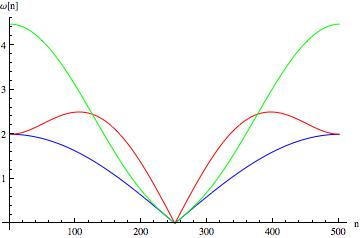
\includegraphics[height=0.7\linewidth,width=\linewidth]{chapter-2/fig/dispersion}
		\caption{subFig 1}
		
	\end{subfigure}
	\begin{subfigure}[h]{0.45\textwidth}
		\centering
		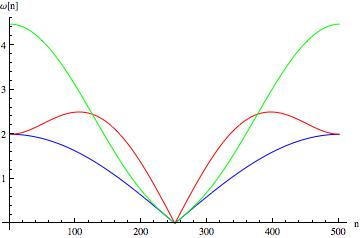
\includegraphics[height=0.7\linewidth,width=\linewidth]{chapter-2/fig/dispersion}
		\caption{subFig 2}
		
	\end{subfigure}
	\centering
	\begin{subfigure}[h]{0.45\textwidth}
		\centering
		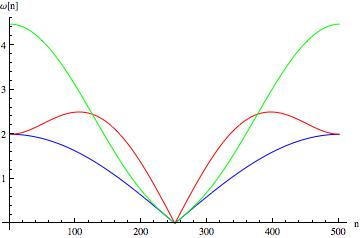
\includegraphics[height=0.7\linewidth,width=\linewidth]{chapter-2/fig/dispersion}
		\caption{subFig 2}
		
	\end{subfigure}
	\caption{All subfigures are together}
	\label{multfig}

\end{figure}
\FloatBarrier
	
You can modify the sizes and shapes of the subfigures as you wish and depending on your preference for the position of these figures with the "htb!" commands. You can use packages like \textbackslash FloatBarrier to prevent \LaTeX from pushing the figures to other pages.


%\newpage





\chapter{}\label{}
Lorem ipsum dolor sit amet, consectetur adipiscing elit, sed do eiusmod tempor incididunt ut labore et dolore magna aliqua. Convallis aenean et tortor at risus viverra adipiscing at. Rutrum tellus pellentesque eu tincidunt tortor aliquam nulla facilisi cras. Luctus accumsan tortor posuere ac ut consequat semper viverra nam. Lectus nulla at volutpat diam ut venenatis tellus in metus. Nibh mauris cursus mattis molestie a iaculis at. Egestas quis ipsum suspendisse ultrices gravida dictum fusce. Lacinia at quis risus sed. Ut venenatis tellus in metus vulputate. Tortor at risus viverra adipiscing. Aliquam vestibulum morbi blandit cursus risus at ultrices. Neque volutpat ac tincidunt vitae. In massa tempor nec feugiat.
\section{Introduction}
Lorem ipsum dolor sit amet, consectetur adipiscing elit, sed do eiusmod tempor incididunt ut labore et dolore magna aliqua. Convallis aenean et tortor at risus viverra adipiscing at. Rutrum tellus pellentesque eu tincidunt tortor aliquam nulla facilisi cras. Luctus accumsan tortor posuere ac ut consequat semper viverra nam. Lectus nulla at volutpat diam ut venenatis tellus in metus. Nibh mauris cursus mattis molestie a iaculis at. Egestas quis ipsum suspendisse ultrices gravida dictum fusce. Lacinia at quis risus sed. Ut venenatis tellus in metus vulputate. Tortor at risus viverra adipiscing. Aliquam vestibulum morbi blandit cursus risus at ultrices. Neque volutpat ac tincidunt vitae. In massa tempor nec feugiat.



 












\chapter{}\label{chap:rf}

Lorem ipsum dolor sit amet, consectetur adipiscing elit, sed do eiusmod tempor incididunt ut labore et dolore magna aliqua. Convallis aenean et tortor at risus viverra adipiscing at. Rutrum tellus pellentesque eu tincidunt tortor aliquam nulla facilisi cras. Luctus accumsan tortor posuere ac ut consequat semper viverra nam. Lectus nulla at volutpat diam ut venenatis tellus in metus. Nibh mauris cursus mattis molestie a iaculis at. Egestas quis ipsum suspendisse ultrices gravida dictum fusce. Lacinia at quis risus sed. Ut venenatis tellus in metus vulputate. Tortor at risus viverra adipiscing. Aliquam vestibulum morbi blandit cursus risus at ultrices. Neque volutpat ac tincidunt vitae. In massa tempor nec feugiat.




\section{Introduction}
Lorem ipsum dolor sit amet, consectetur adipiscing elit, sed do eiusmod tempor incididunt ut labore et dolore magna aliqua. Convallis aenean et tortor at risus viverra adipiscing at. Rutrum tellus pellentesque eu tincidunt tortor aliquam nulla facilisi cras. Luctus accumsan tortor posuere ac ut consequat semper viverra nam. Lectus nulla at volutpat diam ut venenatis tellus in metus. Nibh mauris cursus mattis molestie a iaculis at. Egestas quis ipsum suspendisse ultrices gravida dictum fusce. Lacinia at quis risus sed. Ut venenatis tellus in metus vulputate. Tortor at risus viverra adipiscing. Aliquam vestibulum morbi blandit cursus risus at ultrices. Neque volutpat ac tincidunt vitae. In massa tempor nec feugiat.


\section{ }

Lorem ipsum dolor sit amet, consectetur adipiscing elit, sed do eiusmod tempor incididunt ut labore et dolore magna aliqua. Convallis aenean et tortor at risus viverra adipiscing at. Rutrum tellus pellentesque eu tincidunt tortor aliquam nulla facilisi cras. Luctus accumsan tortor posuere ac ut consequat semper viverra nam. Lectus nulla at volutpat diam ut venenatis tellus in metus. Nibh mauris cursus mattis molestie a iaculis at. Egestas quis ipsum suspendisse ultrices gravida dictum fusce. Lacinia at quis risus sed. Ut venenatis tellus in metus vulputate. Tortor at risus viverra adipiscing. Aliquam vestibulum morbi blandit cursus risus at ultrices. Neque volutpat ac tincidunt vitae. In massa tempor nec feugiat.


\chapter{}
Lorem ipsum dolor sit amet, consectetur adipiscing elit, sed do eiusmod tempor incididunt ut labore et dolore magna aliqua. Convallis aenean et tortor at risus viverra adipiscing at. Rutrum tellus pellentesque eu tincidunt tortor aliquam nulla facilisi cras. Luctus accumsan tortor posuere ac ut consequat semper viverra nam. Lectus nulla at volutpat diam ut venenatis tellus in metus. Nibh mauris cursus mattis molestie a iaculis at. Egestas quis ipsum suspendisse ultrices gravida dictum fusce. Lacinia at quis risus sed. Ut venenatis tellus in metus vulputate. Tortor at risus viverra adipiscing. Aliquam vestibulum morbi blandit cursus risus at ultrices. Neque volutpat ac tincidunt vitae. In massa tempor nec feugiat.

\section{Introduction}
Lorem ipsum dolor sit amet, consectetur adipiscing elit, sed do eiusmod tempor incididunt ut labore et dolore magna aliqua. Convallis aenean et tortor at risus viverra adipiscing at. Rutrum tellus pellentesque eu tincidunt tortor aliquam nulla facilisi cras. Luctus accumsan tortor posuere ac ut consequat semper viverra nam. Lectus nulla at volutpat diam ut venenatis tellus in metus. Nibh mauris cursus mattis molestie a iaculis at. Egestas quis ipsum suspendisse ultrices gravida dictum fusce. Lacinia at quis risus sed. Ut venenatis tellus in metus vulputate. Tortor at risus viverra adipiscing. Aliquam vestibulum morbi blandit cursus risus at ultrices. Neque volutpat ac tincidunt vitae. In massa tempor nec feugiat.

\chapter{Conclusions and future work}

Lorem ipsum dolor sit amet, consectetur adipiscing elit, sed do eiusmod tempor incididunt ut labore et dolore magna aliqua. Convallis aenean et tortor at risus viverra adipiscing at. Rutrum tellus pellentesque eu tincidunt tortor aliquam nulla facilisi cras. Luctus accumsan tortor posuere ac ut consequat semper viverra nam. Lectus nulla at volutpat diam ut venenatis tellus in metus. Nibh mauris cursus mattis molestie a iaculis at. Egestas quis ipsum suspendisse ultrices gravida dictum fusce. Lacinia at quis risus sed. Ut venenatis tellus in metus vulputate. Tortor at risus viverra adipiscing. Aliquam vestibulum morbi blandit cursus risus at ultrices. Neque volutpat ac tincidunt vitae. In massa tempor nec feugiat.



























\begin{appendices}




\end{appendices}
\begin{thebibliography}{99}






\end{thebibliography}


\end{document}